\section{Results}
\subsection{Summary}
In summary, for a two-dimensional cylinder of radius $L$ located at the origin, with steady, inviscid and incompressible fluid flow approaching
in the direction of $\ihat$, with uniform velocity $U\ihat$ infinitely far from the cylinder, in a polar coordinate system:
\begin{align*}
	\phi:r,\theta&\mapsto U\left(r+\frac{L^2}{r}\right)\cos\theta\\
	\vec{V}:r,\theta&\mapsto\left\{\begin{matrix}
		\rhat\left(U-\frac{UL^2}{r^{2}}\right)\cos\theta-\thetahat\left(U+\frac{UL^2}{r^{2}}\right)\sin\theta&r\geq L\\
		\vec{0}&r<L
	\end{matrix}\right.\\
	P:r,\theta&\mapsto\left\{\begin{matrix}
		P_\infty+U^2\left(\frac{L^2}{r^2}\cos2\theta-\frac{L^4}{2r^4}\right) & r\geq L\\
		P_\infty+\frac{\rho U^2}{2} & r<L
	\end{matrix}\right.
\end{align*}
and for a Cartesian coordinate system:
\begin{align*}
	\phi:x,y&\mapsto Ux+\frac{UL^2x}{x^2+y^2}\\
	\vec{V}:x,y&\mapsto\left\{\begin{matrix}
		U\left(1+L^2\frac{y^2-x^2}{\left(x^2+y^2\right)^2}\right)\ihat-UL^2\frac{2xy}{(x^2+y^2)^2}\jhat&x^2+y^2\geq L^2\\
		\vec{0}&x^2+y^2<L^2
	\end{matrix}\right.\\
	P:x,y&\mapsto\left\{\begin{matrix}
		P_\infty+U^2\rho\left(\frac{2L^2\left(x^2-y^2\right)-L^4}{2\left(x^2+y^2\right)^2}\right) & x^2+y^2\geq L^2\\
		P_\infty+\frac{\rho U^2}{2} & x^2+y^2<L^2
	\end{matrix}\right.
\end{align*}

\subsection{Discussion \& visualisations}
\subsubsection{The velocity potential}
The velocity potential $\phi$ is a scalar field whose gradient is equivalent to the velocity field $\vec{V}$. This quantity has no
physical interpretation, but it can be noted that it is a superposition of elementary flow components, namely uniform flow and a dipole. Plotting $\phi$\referto{Figure}{figure:VELOCITY-POTENTIAL} shows lower values (blue) on the left, and higher
values (red) on the right with approximately linear change between them. The plot of $z=\phi$\referto{figure}{figure:VELOCITY-POTENTIAL-3D}
also clearly demonstrates the linear positive change along the $x$ axis, whilst also showing the divergent extremity at $r=0$.
\begin{figure}
	\centering
	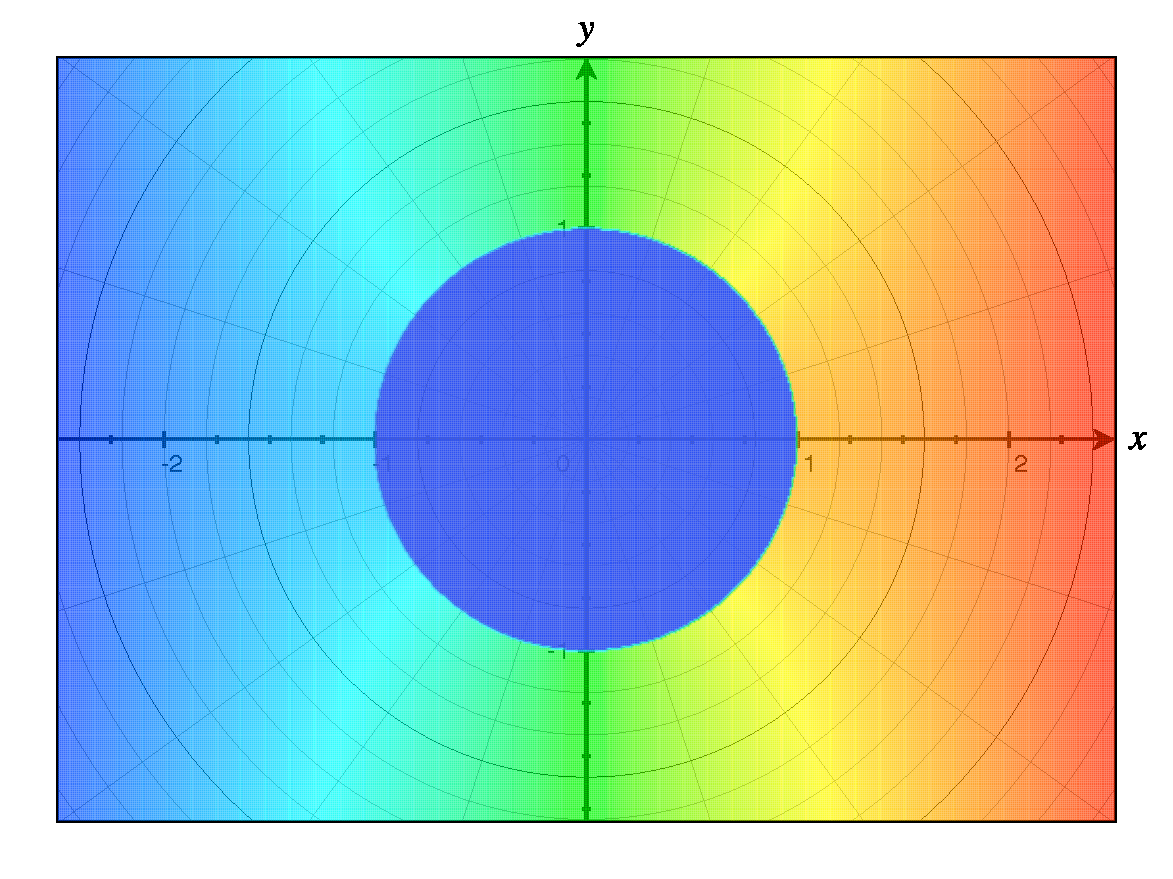
\includegraphics[scale=0.4]{POTENTIAL.pdf}
	\caption{Velocity potential plotted for $L=1$. Blue represents lower values and red represents higher values. Note that all values at coordinates $r<L$ were set to $-3$ to make a readable plot. The value at each point is relative to $U$.}
	\label{figure:VELOCITY-POTENTIAL}
\end{figure}
\begin{figure}
	\centering
	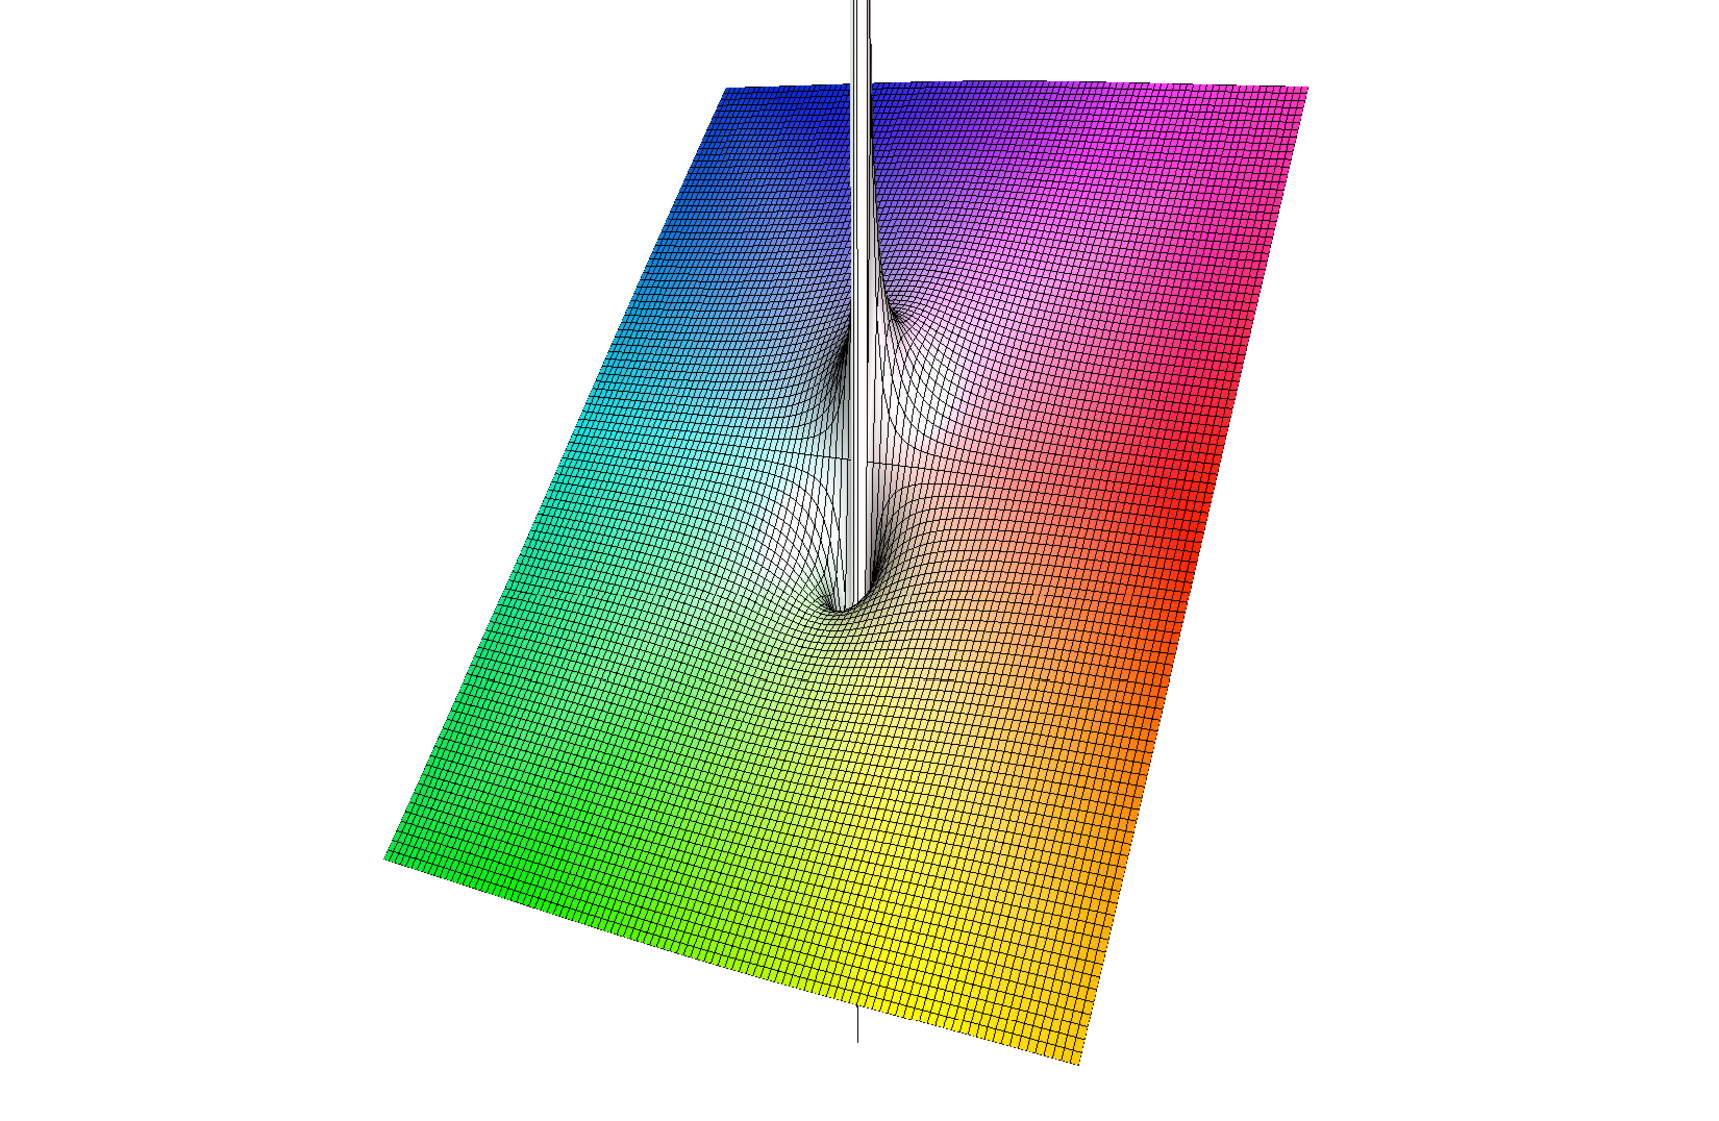
\includegraphics[scale=0.55]{POTENTIAL_Z.pdf}
	\caption{Plot of $z=\phi$, clearly demonstrating the divergent extreme point at $r=0$}
	\label{figure:VELOCITY-POTENTIAL-3D}
\end{figure}

\subsubsection{The velocity field}
The velocity field $\vec{V}$ reveals key insights into the flow modelled. Particularly, there exist two
stagnation points at which the velocity is $\vec{0}$. These exist at $\theta=\frac{\pi}{2}\pm\frac{\pi}{2},\,r=L$.
\begin{align*}
	\vec{V}\left(L, \frac{\pi}{2}\pm\frac{\pi}{2}\right)&=\rhat\left(U-\frac{UL^2}{L^{2}}\right)\cos\left(\frac{\pi}{2}\pm\frac{\pi}{2}\right)-\thetahat\left(U+\frac{UL^2}{L^{2}}\right)\sin\left(\frac{\pi}{2}\pm\frac{\pi}{2}\right)\\
	&=\pm\left(U-\frac{UL^2}{L^{2}}\right)\rhat-0\thetahat\\
	&=\pm\left(U-U\right)\rhat\\
	&=0\rhat-0\thetahat=\vec{0}
\end{align*}
This behaviour is further confirmed by a simple fluid simulation, as seen in Figure~\ref{figure:FSIM} (for more information on the simulation, refer to the appendix, Section~\ref{section:FSIM}).
Conversely, as illustrated by a plot of the velocity field\referto{Figure}{figure:VELOCITY_FIELD}, the fluid is accelerated over the top and bottom ($\theta=\pm\frac{\pi}{2}$), where the fluid reaches
its highest speed.
\begin{figure}
	\centering
	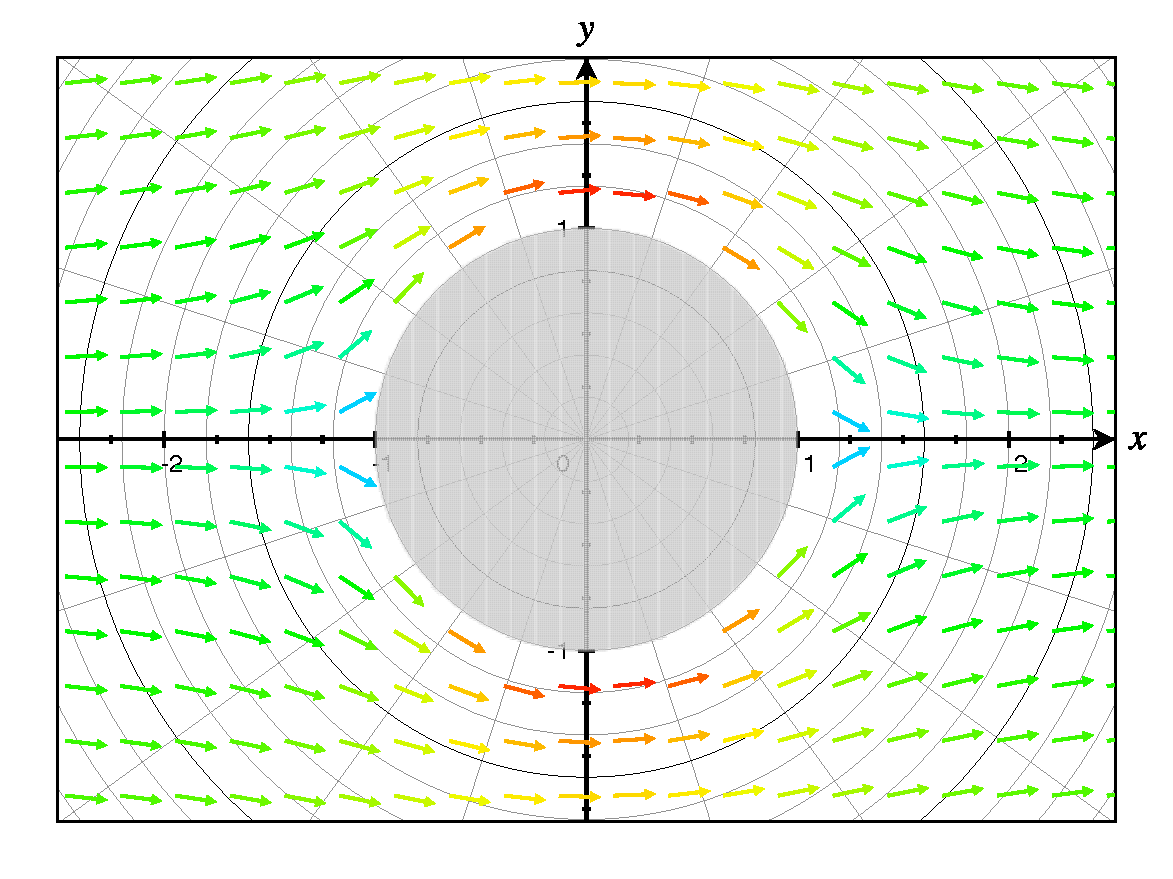
\includegraphics[scale=0.5]{VELOCITY.pdf}
	\caption{Velocity field plotted for and $L=1$. Blue represents lower speed and red represents higher speed. The magnitude of the arrows are relative to $U$.}
	\label{figure:VELOCITY_FIELD}
\end{figure}
\begin{figure}
	\centering
	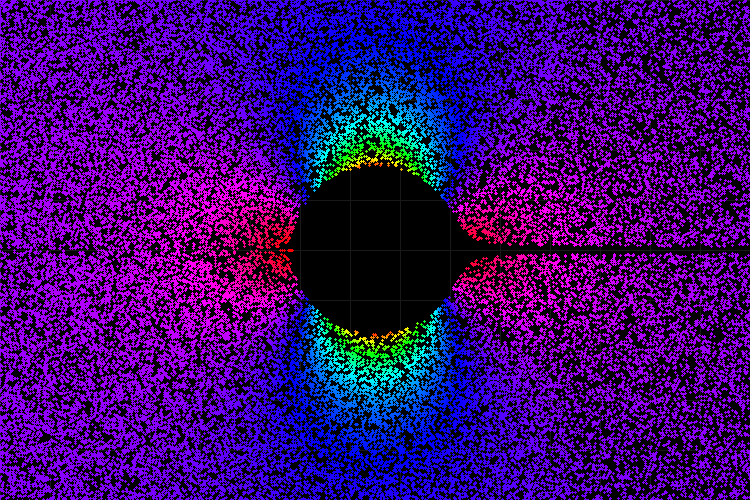
\includegraphics[scale=0.5]{FSim_frame_1.png}
	\caption{Selected frame from a fluid simulation showing a fluid parcel stuck at a stagnation point. The wake behind the cylinder is an artefact of the simulation code (for more information, refer to the appendix, Section~\ref{section:FSIM}) and whilst a normal physical phenomenon, is not captured by the idealised model derived in this essay. Red represents lower speed, green represents higher speed.}
	\label{figure:FSIM}
\end{figure}

\subsubsection{The pressure field}
Bernoulli's principle states an inverse relationship between pressure and velocity. Thus the pressure is the highest at the stagnation points,
and lowest at the top and bottom. This is visually confirmed by Figures \ref{figure:pressure:1} and \ref{figure:pressure:2}. As seen in these figures,
the pressure distribution is symmetric, leading to the surprising paradoxical result, known as d'Alembert's paradox, where the drag force acting on the cylinder is $0$.
\begin{figure}
	\centering
	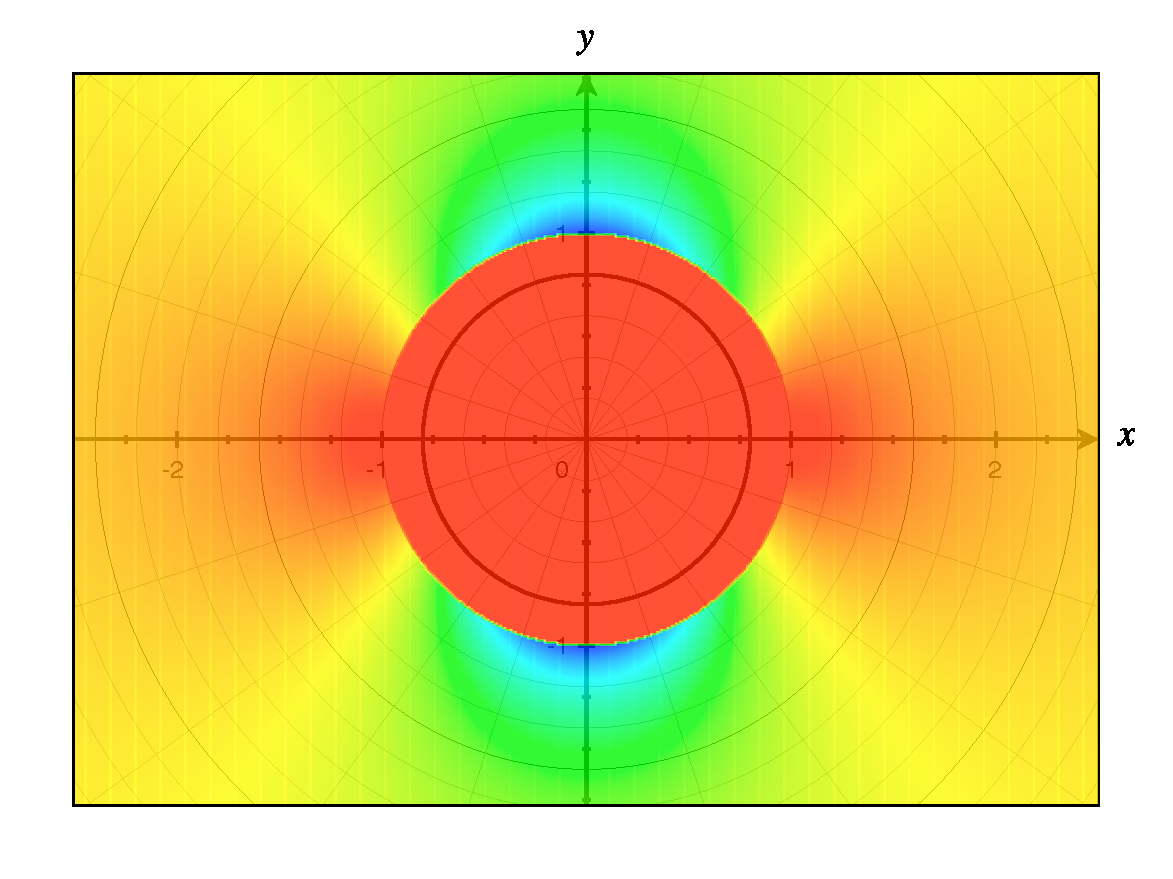
\includegraphics[scale=0.5]{pressure.pdf}
	\caption{Pressure field plotted for $L=1$. Blue represents lower pressure and red represents higher pressure. The pressure at each point is relative to $U$.}
	\label{figure:pressure:1}
\end{figure}
\begin{figure}
	\centering
	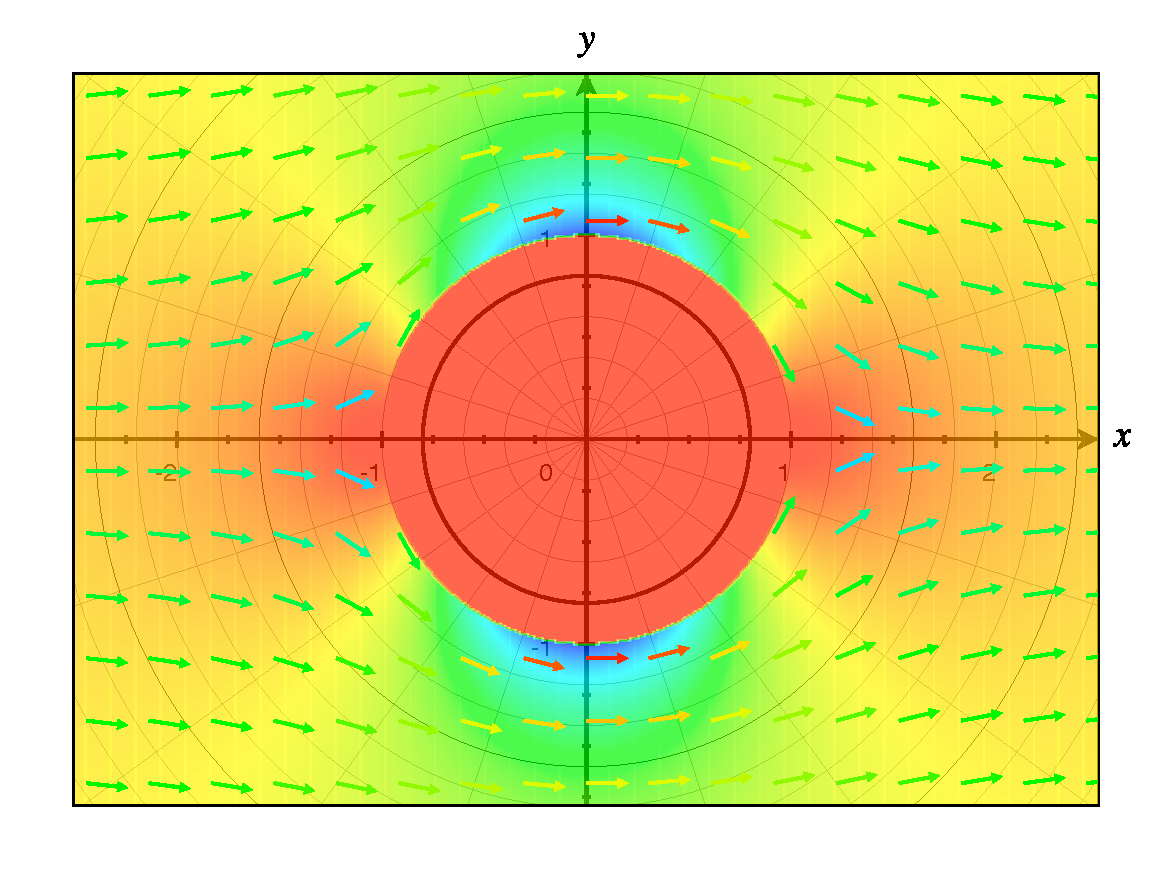
\includegraphics[scale=0.5]{pressure_velocity.pdf}
	\caption{Pressure field plotted for $L=1$. Blue represents lower pressure and speed, red represents higher pressure and speed. The pressure at each point is relative to $U$.}
	\label{figure:pressure:2}
\end{figure}

\section{Conclusion}
In this essay, the fundamental principles of vector calculus were used to model the steady, incompressible, and inviscid flow of a fluid past a cylinder.
Through the velocity potential, given by the solving of Laplace's equation, the pressure- and velocity-fields could be derived, providing a complete 
description of the fluid's behaviour. The model derived successfully predicts key phenomena, such as the existance of stagnation points at the front and
back of the cylinder, as well as the inverse relationship between pressure and speed as described by Bernoulli's principle. While this idealised model
leads to the paradoxical result of zero drag force and lacks key physical phenomena such as wakes which form in viscous fluid, it can serve as a crucial
foundation for understanding more complex fluid dynamics.